\chapter{Neutrino  experiments}
\label{c:expIntro}

This chapter is aimed at putting the babyMIND experiment into context of what has been done before, what experiments are underway and what experiments are planned.

\section{Previous important neutrino detector experiments}

This section details some of the important previous neutrino experiments that have take place. The different experiments can be split into three different categories based on the primary neutrino source
The detector types are:
\begin{itemize}
\item Accelerator
\item Atmospheric/Cosmic
\item Reactor
\end{itemize}
Each will be described briefly before examples are given.

\subsection{Accelerator}
Can produce either muon or electron normal or anti neutrinos.
Produced from inverse beta decay? Stars off from proton beam. Continues. Finally uses a magnetic horn to split the positive and negative. Then allow for interaction to neutrinos.

Advantage, energy range well known.

\subsubsection{K2K / T2-K}
After the success of Super-Kamiokande, the K2K-experiment\cite{22K2K} was created with the main difference of using a well understood muon neutrino beam pointing at the Super-Kamiokande detector at a distance of 250 km. It was the first neutrino oscillation measurement where both the source and detector were controlled, it observed the disappearance of muon neutrinos and found results that were consistent with Super-Kamiokande.

The next improvement came with the T2K-experiment\cite{21T2K}, which was also a long-baseline neutrino oscillation experiment with a more powerful beam from the JPARC facility to Super-Kamiokande, at a distance of 295 km. The experiment wanted to improve the understanding of the neutrino oscillation parameters. T2K was able to successfully observe the appearance of muon to electron neutrino oscillations and find evidence that the third mixing angle $\theta_{13}$ is not zero. This is still an ongoing experiment.
\subsubsection{MINOS}
MINOS~\cite{MINOS} is also a muon neutrino disappearance experiment, consisting of one near and one far detector and using the NuMI~\cite{19NuMI} beam at Fermilab, to better understand the neutrino beam and showed results consistent with Super-Kamiokande and the K2K experiments.
\subsubsection{NOvA}
After MINOS the next step using the NuMI~\cite{19NuMI} beam is the NOvA~\cite{18nova} experiment, which is also an electron neutrino appearance experiment and hopes to be able to determine the mass hierarchy of neutrinos.
\subsubsection{MINERvA}
\subsubsection{MiniBooNE}

\subsection{Atmospheric/Cosmic}
Using naturally occurring neutrinos produced from stars etc.

Advantage, very high energy, very large distance and can use the earth to remove background.

\subsubsection{SNO}
\subsubsection{Kamiokande}
\subsubsection{KamLAND}
\subsubsection{Super-K}
Super-Kamiokande\cite{20SUPERK}, an upgraded version of the Kamiokande water Cherenkov detector performed the first experimental observation that the neutrino has non-zero mass\cite{10Fukuda} and also managed to detect strong evidence of muon neutrino oscillation to tau neutrinos from the analysis of atmospheric neutrinos interacting in the water Cherenkov target.
\subsubsection{IceCube}

\subsection{Reactor}
Beta decay all the way? Can produce very low energy neutrinos. 


\subsubsection{Daya Bay}
\subsubsection{Double Chooz}
\subsubsection{KamLAND}
\subsubsection{RENO}

\subsection{Summary of important discoveries}
\textbf{Table, different mass and so on.}
\subsection{Current limits}

\section{Future neutrino experiments}
\subsection{KATRIN}
\subsection{Hyper-K}
The Hyper-Kamiokande Experiment\cite{24HyperK}  builds on the T2K-experiment\cite{21T2K} by improving the neutrino beam at JPARC, and building a 500 kton water Cherenkov detector, which aims to improve the sensitivity for $\delta_{cp}$.
\subsection{DUNE}
LBNF/DUNE\cite{23DUNE} is a new experiment aiming at looking at the full range of $\delta_{cp}$ with greater sensitivity than before by improving on the MINOS~\cite{MINOS} experiment, and performing an electron neutrino appearance measurement with a high-powered neutrino beam from Fermilab and a 40 kton liquid argon detector at a distance of 1300 km, in the Homestake mine in South Dakota.
\subsection{nuStorm experiment}
\subsection{Neutrino factory}
One concept to achieve a high number of neutrino events from a well-understood neutrino beam is the so called Neutrino Factory~\cite{25NUfact}, which will create a high number of electron and muon neutrino events from the decay of high-energy muons.

A nuSTORM facility, which could be seen as the first stage towards a neutrino factory, is expected to have sensitivity for sterile neutrinos with a MIND type detector\cite{29nuSTORM} upto 10$\sigma$ compared to previous measurements.
\begin{figure}[h!]
\centering
\includegraphics[width=\textwidth]{figures/nuSTORM_schematic.pdf}
\caption{A schematic of a nuSTORM facility~\cite{Fix7}.}
\label{fig:nuStorm}
\end{figure}

The neutrino factory has the capacity to improve the precision of neutrino oscillation measurements, since the neutrino beam from the decay of muons can be determined with high accuracy. The beam produces one bunch of $\mu^+$ and one bunch of $\mu^-$, so the facility can make measurements of $\nu_{\mu}$ and $\bar{\nu_{e}}$ and $\bar{\nu_{\mu}}$ and $\nu_{e}$ simultaneously. Using this $\delta_{cp}$ can be decisively explored, with an expected accuracy of $\Delta \delta_{CP}\sim 5^\circ$~\cite{25NUfact}.

\begin{figure}[h!]
\centering
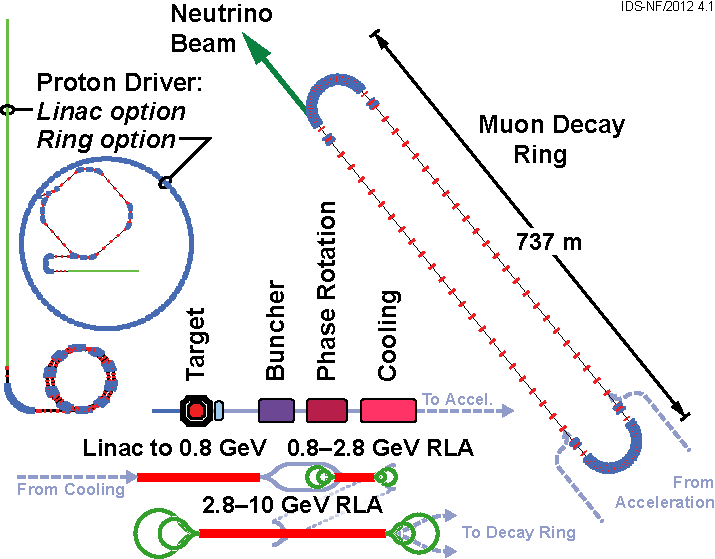
\includegraphics[width=0.9\textwidth]{figures/131112-IDS-NF.pdf}
\caption{Schematic diagram of the Neutrino Factory~\cite{Fix7}.}
\label{fig:nuFact}
\end{figure}

\begin{figure}[h!]
\centering
\includegraphics[width=0.9\textwidth]{figures/rdr-cp-precision-comparison-131216.pdf}
\caption{Expected precision for a measurement of the $\delta_{cp}$ at a Neutrino Factory compared to alternate neutrino oscillation facilities~\cite{Fix7}.}
\label{fig:nuFactExp}
\end{figure}

%==============================================================================
